% Präambel
\documentclass[12pt,			% Schriftgröße
a4paper,						% Papierformat
twoside, 						% einseitiges (oneside) oder zweiseitiges (twoside) Dokument
listof=totoc, 					% Tabellen- und Abbildungsverzeichnis ins Inhaltsverzeichnis
bibliography=totoc,				% Literaturverzeichnis ins Inhaltsverzeichnis aufnehmen
titlepage, 						% Titlepage-Umgebung statt \maketitle
headsepline, 					% horizontale Linie unter Kolumnentitel
%abstracton,					% Überschrift beim Abstract einschalten, Abstract muss dazu in {abstract}-Umgebung stehen
DIV18,							% auskommentieren, um den Seitenspiegel zu vergrößern
BCOR6mm,						% Bindekorrektur, die den Seitenspiegel um 6mm nach rechts verschiebt,
cleardoublepage=empty,			% Stil einer leeren eingefügten Seite bei Kapitelwechsel
parskip,						% Absatzabstand bei Absatzwechsel einfügen
ngerman							% Übersetzung der festcodierten Überschriften
]{scrbook}			
\usepackage{ucs} 				% Dokument in utf8-Codierung schreiben und speichern
\usepackage{babel} 				% deutsche Trennungsregeln
\usepackage[utf8x]{inputenc} 	% ermöglicht die direkte Eingabe von Umlauten
\usepackage[T1]{fontenc} 		% Ausgabe aller zeichen in einer T1-Codierung (wichtig für die Ausgabe von Umlauten!)
\setlength{\parindent}{0ex} 	% bei neuem Abschnitt nicht einrücken
\linespread{1.2}\selectfont     % Zeilenabstand erhöhen - größere Werte als 1.2 nicht verwenden!!
\usepackage{scrpage2}			% SCR Headings verwenden
\setheadsepline{0.4pt}			% Kopfzeile Linien oben
\setfootsepline{0.4pt}			% Kopfzeile Linien unten
\pagestyle{scrheadings}			% SCR Headings einschalten
\usepackage{graphicx}  			% Einbinden von Grafiken erlauben
\usepackage[format=hang,		% Formatierungen von Unter- / Überschriften
font=normal,
labelfont=bf,
justification=RaggedRight,
singlelinecheck=true,
aboveskip=1mm
]{caption}

\usepackage{enumitem}			% Erlaubt Änderung der Nummerierung in der Umgebung enumerate

\usepackage{amsmath}			% Ergänzungen für Formeln
\usepackage{textcomp} 			% zum Einsatz von Eurozeichen u. a. Symbolen
\usepackage[%
%per=slash,
decimalsymbol=comma,
%thickspace,					
%thickqspace
]{siunitx}						% Einfache Eingabe von SI-Einheiten
\sisetup{number-unit-product = \;, inter-unit-product = \:}
\newcommand*\diff{\mathop{}\!\mathrm{d}}	% Differentialzeichen
\newcommand*\Diff[1]{\mathop{}\!\mathrm{d^#1}} % Differentialzeichen höherer Ableitung
\newcommand*\jj{\mathop{}\!\mathrm{j}}	% Komplexe Zahl j

\usepackage[					% Einstellunge Paket hyperref
hyperfootnotes=false			% im pfd-Output Fußnoten nicht verlinken
]{hyperref}

\usepackage{makeidx}			% Paket zur Erstellung eines Index
\usepackage[printonlyused]{acronym} 	% zur Erstellung des Abkürzungsberzeichnisses

\usepackage[					% Einstellungen für Fußnoten
bottom,							% Ausrichtung unten
multiple,						% Trennung durch Seperator bei mehreren Fußnoten
hang,
marginal
]{footmisc}

\usepackage{calc}				% Paket zum Berechnen von Längen z.B. 0.8\linewidth

\usepackage{xcolor} 			% einfache Verwendung von Farben in nahezu allen Farbmodellen

\usepackage{listings}			% Darstellung von Quellcode mit den Umgebungen {lstlisting}, \lstinline und \lstinputlisting
\lstset{literate=				% Damit können Umlaute innerhalb Listings geschrieben werden
	{Ö}{{\"O}}1
	{Ä}{{\"A}}1
	{Ü}{{\"U}}1
	{ß}{{\ss}}1
	{ü}{{\"u}}1
	{ä}{{\"a}}1
	{ö}{{\"o}}1
}

%****************************************************************** Zusätzliche Packages *******************
%*****************************************************

\usepackage{color}
\usepackage{colortbl}
\usepackage{pdfpages}

%*****************************************************************************************************************************************************************

\definecolor{mygreen}{rgb}{0,0.6,0}
\definecolor{mygray}{rgb}{0.5,0.5,0.5}
\definecolor{mymauve}{rgb}{0.58,0,0.82}
\lstset{ %
	backgroundcolor=\color{white},   % choose the background color; you must add \usepackage{color} or \usepackage{xcolor}; should come as last argument
	basicstyle=\footnotesize,        % the size of the fonts that are used for the code
	breakatwhitespace=false,         % sets if automatic breaks should only happen at whitespace
	breaklines=true,                 % sets automatic line breaking
	captionpos=t,                    % sets the caption-position to (b) bottom or (t) top
	commentstyle=\color{mygreen},    % comment style
	deletekeywords={...},            % if you want to delete keywords from the given language
	escapeinside={\%*}{*)},          % if you want to add LaTeX within your code
	escapeinside={(*@}{@*)},
	extendedchars=true,              % lets you use non-ASCII characters; for 8-bits encodings only, does not work with UTF-8
	frame=none,	                   	% "single" adds a frame around the code; "none"
	keepspaces=true,                 % keeps spaces in text, useful for keeping indentation of code (possibly needs columns=flexible)
	keywordstyle=\color{blue},       % keyword style
	language=[LaTeX]TeX,             % the language of the code
	morekeywords={*,nomenclature},   % if you want to add more keywords to the set
	numbers=left,                    % where to put the line-numbers; possible values are (none, left, right)
	numbersep=5pt,                   % how far the line-numbers are from the code
	numberstyle=\tiny\color{mygray}, % the style that is used for the line-numbers
	rulecolor=\color{black},         % if not set, the frame-color may be changed on line-breaks within not-black text (e.g. comments (green here))
	showspaces=false,                % show spaces everywhere adding particular underscores; it overrides 'showstringspaces'
	showstringspaces=false,          % underline spaces within strings only
	showtabs=false,                  % show tabs within strings adding particular underscores
	stepnumber=1,                    % the step between two line-numbers. If it's 1, each line will be numbered
	stringstyle=\color{mymauve},     % string literal style
	tabsize=2,	                   % sets default tabsize to 2 spaces
	title=\lstname                   % show the filename of files included with \lstinputlisting; also try caption instead of title
}

\makeindex						% Indexverzeichnis erstellen
				% Abkürzungsverzeichnis erstellen

% -----------------------------------------------------------------------------------------------------------------
% Zum Aktualisieren des Abkürzungsverzeichnisses (Nomenklatur) bitte auf der Kommandozeile folgenden Befehl aufrufen :
% makeindex <Dateiname>.nlo -s nomencl.ist -o <Dateiname>.nls
% Oder besser: Kann in TexStudio unter Tools-Benutzer als Shortlink angelegt werden
% Konfiguration unter: Optionen-Erzeugen-Benutzerbefehle: makeindex -s nomencl.ist -t %.nlg -o %.nls %.nlo
% -----------------------------------------------------------------------------------------------------------------

% Hier die persönlichen Daten eingeben:

\newcommand{\titel}{ProjektB-Elektrik}
\newcommand{\untertitel}{}
\newcommand{\arbeit}{Simulationstechnik - Bericht}
\newcommand{\studiengang}{Elektrotechnik}
\newcommand{\studienrichtung}{Fahrzeugelektronik}
\newcommand{\autor}{Alexander Herrmann, Johannes Ruffer}
\newcommand{\matrikelnr}{9859538 x 1011921}
\newcommand{\kurs}{TFE18-2}
\newcommand{\abgabe}{19.04.2020}
\newcommand{\zeitraum}{01.02.2020 - 19.04.2020}
\newcommand{\betreuerdhbw}{Sipler}
\newcommand{\jahr}{2020}			% für Angabe im Copyright-Vermerk der Titelseite

% Folgende Zeilen definieren Abkürzungen, um Befehle schneller eingeben zu können
\newcommand{\ua}{\mbox{u.\,a.\ }}
\newcommand{\zB}{\mbox{z.\,B.\ }}
\newcommand{\bs}{$\backslash$}

% Folgende Zeilen weden benötigt, um Tikz und PGF-Plot-Grafiken einzubinden
\usepackage{pgfplots}
\usepackage{pgfplotstable}
\pgfplotsset{compat=newest,width=0.6\linewidth}
\usepgfplotslibrary{smithchart}
\usepackage{tikz}						% Tikz sollte nach Listings Pakete geladen werden.
\usetikzlibrary{arrows}
\usetikzlibrary{positioning,shadings}


%\usepackage{pgfkeys,pgfmath,pgfcore}% or pgf or tikz or pgfplots
%
%\pgfkeys{
%	/pgf/number format/textnumber/.style={
%		fixed,
%		use comma,
%		fixed zerofill,
%		precision=4,
%		1000 sep={.},
%	},
%}


\hyphenation{Schrift-ar-ten}

%\renewcommand\thesection{~\arabic{section}}



% -------------------------------------------------------------------------------------------
%                     Beginn des Dokumenteninhalts
% -------------------------------------------------------------------------------------------
\begin{document}
\setcounter{secnumdepth}{3}				% Nummerierungstiefe fürs Inhaltsverzeichnis
\setcounter{tocdepth}{3}
\sffamily								% für die Titelei serifenlose Schrift verwenden

% ------------------------------ Titelei -----------------------------------------------------

\thispagestyle{plain}
\begin{titlepage}
\enlargethispage{4.0cm}
\sffamily 								% Serifenlose Grundschrift für die Titelseite einstellen

\parbox{0.5\linewidth}{
\begin{flushleft}
%\includegraphics[width=0.4\linewidth]{images/Daimler-Logo}\\[5ex]
\end{flushleft}
}
\parbox{0.5\linewidth}{
\begin{flushright}
	
\includegraphics[width=0.4\linewidth]{images/DHBW_d_R_FN_46mm_4c}\\[5ex]
\end{flushright}
}
				

\begin{center}

\LARGE{\textsc{\textbf{\titel}}}\\[1.5ex]
%\Large{\textbf{\untertitel}}\\[5ex]
\Large{\textbf{\arbeit}}\\[2ex]
%\normalsize{für die Prüfung zum\\[1ex] Bachelor of Engineering}\\[3ex]
\Large{Studiengang \studiengang}\\[2ex]
\large{Studienrichtung \studienrichtung}\\[1ex]
\normalsize{Duale Hochschule Baden-Württemberg Ravensburg, Campus Friedrichshafen}\\[5ex]
von\\[1ex] 

\begin{tabular}{cc}
	& \\
	Alexander Herrmann & Johannes Ruffer\\
\end{tabular}


\end{center}

\begin{flushleft}

\begin{tabular}{ll}
Abgabedatum:					& \quad \abgabe \\
Bearbeitungszeitraum:		   		& \quad \zeitraum \\ 
Matrikelnummer: 			& \quad \matrikelnr \\
Kurs: 							& \quad \kurs \\
Gutachter der Dualen Hochschule: & \quad \betreuerdhbw \\ [5ex]

\end{tabular} 



\small
%Copyrightvermerk:\\

%Dieses Werk einschließlich seiner Teile ist \textbf{urheberrechtlich geschützt}. Jede Verwertung außerhalb der engen Grenzen des Urheberrechtgesetzes ist ohne Zustimmung des Autors unzulässig und strafbar. Das gilt insbesondere für Vervielfältigungen, Übersetzungen, Mikroverfilmungen sowie die Einspeicherung und Verarbeitung in elektronischen Systemen.
\end{flushleft}
\begin{flushright}
%\copyright{} \jahr
\end{flushright}
\end{titlepage}

\cleardoublepage 				% erzeugt die Titelseite
\pagenumbering{roman}					% kleine, römische Seitenzahlen für Titelei
\chapter*{Eidesstattliche Erklärung} %*-Variante sorgt dafür, das Abstract nicht im Inhaltsverzeichnis auftaucht

%Mit der Abgabe der Aufgabenlösung in Moodle erklären Sie, dass Sie den Programmentwurf selbständig verfasst und keine anderen als die angegebenen Quellen und Hilfsmittel benutzt haben.

Gemäß Ziffer 1.1.13 der Anlage 1 zu §§ 3, 4 und 5  der Studien- und Prüfungsordnung für die Bachelorstudiengänge im Studienbereich Technik der Dualen Hochschule Baden-Würt­tem­berg vom 29.09.2015.

Wir versichern hiermit, dass wir unsere Projektarbeit mit dem Thema: 

\begin{quote}
	\textit{\titel} \textit{ \untertitel }
\end{quote}

selbstständig verfasst und keine anderen als die angegebenen Quellen und Hilfsmittel benutzt haben. Wir versichern zudem, dass die eingereichte elektronische Fassung mit der gedruckten Fassung übereinstimmt.

Friedrichshafen, den \today \\[2ex]

\begin{center}

\begin{tabular}{cc}
	\rule[-0.2cm]{0.3\linewidth}{0.5pt} & \rule[-0.2cm]{0.3\linewidth}{0.5pt}\\
	Alexander Herrmann & Johannes Ruffer\\
\end{tabular}

\rule{0.75\linewidth}{0.1pt}\\
\textsc{Autoren} \\[10ex]
\end{center}


%Sperrvermerk bei Bedarf dekommentieren
%\hrule 
%\vspace*{1.0cm}
\noindent \textbf{\Large{Sperrvermerk}}\\
\normalsize
Die Ergebnisse der Arbeit stehen ausschließlich dem auf dem Deckblatt aufgeführten Ausbildungsbetrieb zur Verfügung.

\normalsize

\rmfamily



\cleardoublepage 				% Einbinden der eidestattlichen Erklärung

\addchap*{Kurzfassung}
% Kurzfassung - Autor:

\label{kurzfassung}



\tableofcontents						% Erzeugen des Inhalsverzeichnisses
\cleardoublepage

% --------------------------------------------------------------------------------------------
%                    Inhalt der Bachelorarbeit
%---------------------------------------------------------------------------------------------
\pagenumbering{arabic}					% arabische Seitenzahlen für den Hauptteil

\rmfamily

\chapter{Einleitung}
%\setcounter{figure}{0}
\setcounter{chapter}{1}
% Autor:

\label{Einleitung}
In diesem Bericht wird ein Unwuchtsystem im Hinblick auf dessen elektronische Komponente simulationstechnisch betrachtet. Dafür wird der integrierte Gleichstrommotor vereinfacht durch das Ersatzschaltbild einer Nebenschlussmaschine dargestellt. Anhand dieser Vereinfachung wird das System einer Simulationsstudie unterzogen. Hierbei beginnt man das Originalsystem, mittels Systemanalysen und Modellbildung, in Modelle oder Teilsysteme zu überführen in denen leichter gearbeitet werden kann. So zum Beispiel das Mathematische Modell, in diesem werden die einzelnen Differentialgleichungen aufgestellt, die zur Untersuchung des System notwendig sind. Im gleichen Schritt wird das Modell analysiert und dessen Systemeigenschaften, wie Ausgangs- und Eingangsgrößen, erarbeitet. Im vorliegenden System sind die Ausgangsgrößen beispielsweise das Motormoment $M_A$, die Unwuchtkraft $F_U$, die Winkelgeschwindigkeit $\Omega$ und die Strecke $s$. Um diese weiter untersuchen zu können werden die entdeckten Eigenschaften und Systemgleichungen in Matlab implementiert, um dort die gewünschten Simulationen durchzuführen. 

\chapter{Aufgabenteil a.)}


\begin{figure}[hbt]
	\centering
	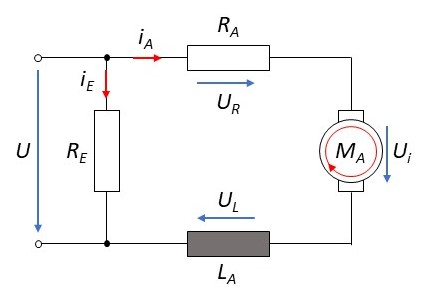
\includegraphics[width=0.5\linewidth]{Images/ProjektB_Elektrik_Ph_Modell_Schaltplan}
	\caption{Physikalisches Modell mit Spannungen und Strömen}
	\label{fig:schaltbild}
\end{figure}

Zu den elektrischen Größen:
\begin{equation*}
\begin{aligned}
&M_A = K_A i_A \\
&P_A = U_i i_A = M_A \omega_A = K_A i_A \omega_A \\
&U_i = K_A \omega_A = K_A \dot{\varphi} \\
&i_E = \frac{U}{R_E}
\end{aligned}
\end{equation*}

Mathematisches Modell der Nebenschlussmaschine:
\begin{equation*}
\begin{aligned}
&U = U_R + U_i + U_L \\
&U = R_A i_A + K_A \dot{\varphi} + L_A \frac{\diff{i_A}}{\diff{t}} \\
&0 = R_A i_A + K_A \dot{\varphi} + L_A \frac{\diff{i_A}}{\diff{t}} - U \\
\end{aligned}
\end{equation*}

Systemgleichung des Umwuchtsystems:
Translatorisch:
\begin{equation}
\begin{aligned}
(m_1 + m_2) \ddot{s} - m_2 e(\ddot{\varphi} \sin{\varphi} + \ddot{\varphi^2} \cos{\varphi}) + d_t \dot{s} + c s &= 0 \\
\ddot{s} = \frac{1}{m_1 + m_2}[m_2 e(\ddot{\varphi} \sin{\varphi} + \ddot{\varphi^2} \cos{\varphi}) - d_t \dot{s} - c s] &= f_1(\varphi, \dot{\varphi}, \ddot{\varphi}, s, \dot{s}) \label{enq:Bewgltrans}
\end{aligned}
\end{equation}
Rotatorisch:
\begin{equation}
\begin{aligned}
m_2 e^2 \dot{\varphi} - m_2 e \sin{\varphi} (\ddot{s} + g) d_r \dot{\varphi} - M_A &= 0 \\
m_2 e^2 \dot{\varphi} - m_2 e \sin{\varphi} (\ddot{s} + g) d_r \dot{\varphi} - K_A i_A &= 0 \\
\ddot{\varphi} = \frac{1}{m_2 e^2} [m_2 e \sin{\varphi} (\ddot{s} + g) d_r \dot{\varphi} + K_A i_A] &= f_2(\varphi, \dot{\varphi}, \ddot{s}, i_A) \label{enq:Bewglrot}
\end{aligned}
\end{equation}

Durch Vernachlässigung des Erregerstroms $i_E$ folgt:
\begin{equation}
\begin{aligned}
U &= i_A R_A + L_A \dot{i_A} + K_A \dot{\varphi} \\
\frac{\diff{i_A}}{\diff{t}} &= \frac{1}{L_A} (U - K_A \dot{\varphi} - i_A R_A) = f_3(U, \dot{\varphi}, i_A)
\end{aligned}
\end{equation}

%Folgesituationen
\begin{figure}[hbt]
	\begin{tikzpicture}
	
	%Zeichnung de Holzblöcke
	\draw (4,0.5) rectangle (9,2.5) node[midway, align=center](Block){Unwuchtsystem}; 
	
	%Pfeile
	\begin{scope}
	\draw[->] (0,1.5) -- (4,1.5);
	\draw[->] (9,1.5) -- (13,1.5);
	\end{scope}
	
	%Parameterbeschriftungen
	\draw(0,2.25) node(uin) {$u = U$};
	\draw(13.75,2.25) node(yvek) {$\underline{y} = \left[\begin{array}{c} s \\\ \dot{\varphi} \\\ M_A \\\ F_U \end{array}\right]$};
	
	\end{tikzpicture}
	
	%Abbildungsunterschrift
	\caption{Unwuchtsystem mit Eingangsspannung und Ausgang (Kinematik, Kinetik)}
	\label{fig:Unwuchtsystem}
	
\end{figure}


\begin{figure}[hbt]
	\centering
	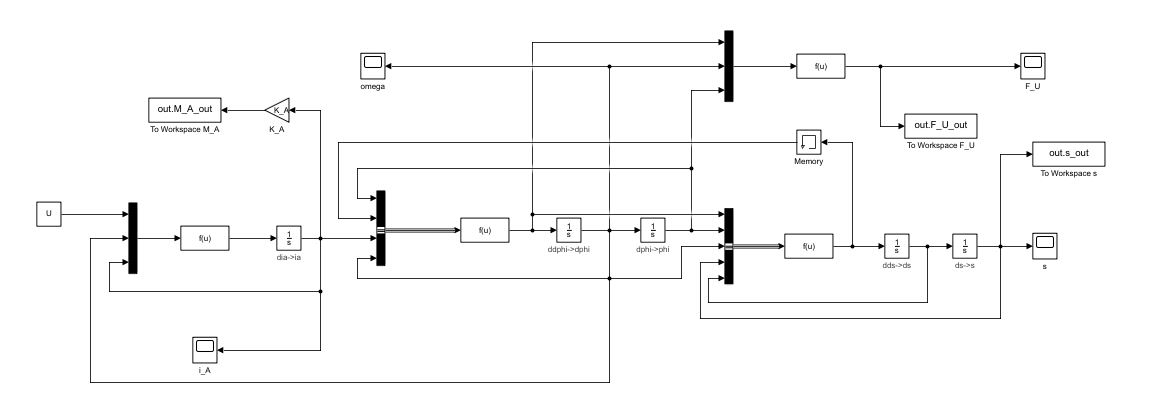
\includegraphics[width=1\linewidth]{Images/ProjektB_Elektrik_Blockdiagramm}
	\caption{SIMULINK Blockdiagramm zur Simulation des Systemverhaltens mit Memory-Block zur Umgehung der algebraischen Schleife}
	\label{fig:Blockdiagramm}
\end{figure}

\begin{figure}[hbt]
	\centering
	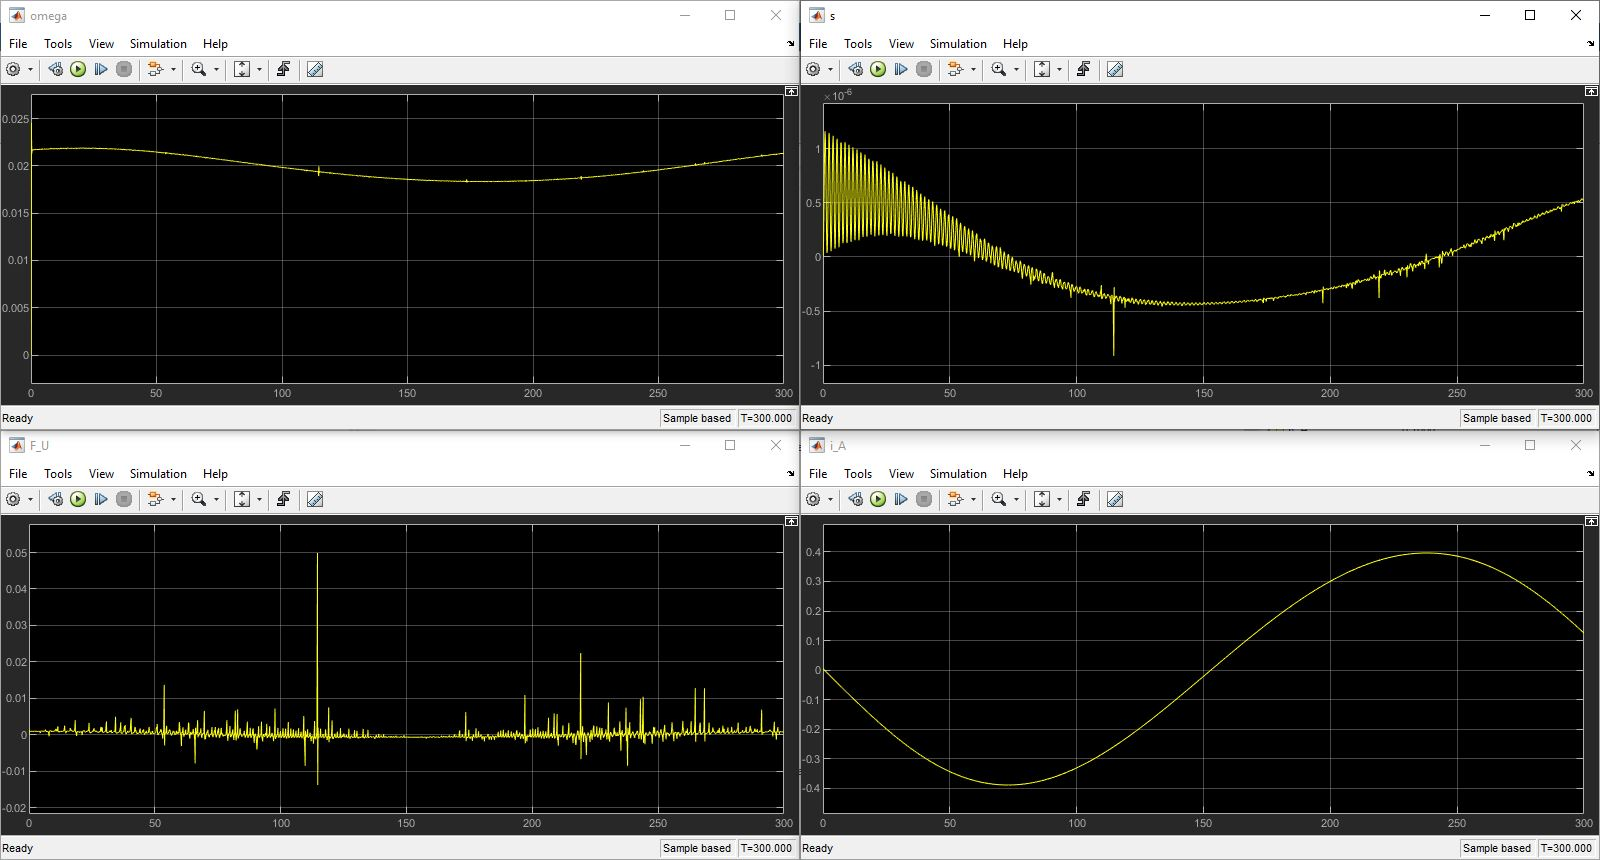
\includegraphics[width=0.5\linewidth]{Images/ProjektB_Elektrik_Diagramme_1}
	\caption{Simulationsergebnisse}
	\label{fig:Simulationsergebnisse}
\end{figure}

\section{Physikalisches Modell}
In Abbildung \ref{fig:Schaltbild} wird der Gleichstrommotor des Umwuchtsystems, vereinfacht durch das physikalische Modell einer Nebenschlussmaschine dargestellt. Diese besteht aus einem Wicklungssystem des Ankerkreises und einer Erregerwicklung, welche dem Motor parallel geschaltet ist. Aufgrund von Wicklungen und Streufeldern im Ankerkreis entsteht eine Induktivität $L_A$, über welche die Spannung $U_L$ abfällt. Dazu ist ein Widerstand $R_A$ geschaltet. Der Gleichstrommotor wird dabei ausschließlich von der Klemmspannung $U$ gesteuert. \\

\begin{figure}[!hbt]
	\centering
	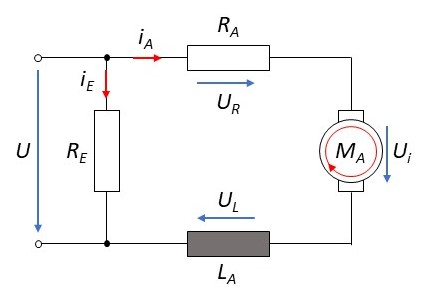
\includegraphics[width=0.5\linewidth]{Images/ProjektB_Elektrik_Ph_Modell_Schaltplan}
	\caption{Physikalisches Modell mit Spannungen und Strömen}
	\label{fig:Schaltbild}
\end{figure}

Die gegebenen Systemparameter lauten dabei:

\begin{table}[!hbt]
	\centering
	
	\begin{tabular}{| l | l |}
		\hline
		Ankerflussverkettung, Motorkonstante & $M_A = 50 \frac{\newton\meter}{\ampere}$ \\
		\hline
		Ohmscher Widerstand des Ankerkreises & $R_A = 0.1 \ohm$ \\
		\hline
		Induktiver Widerstand des Ankerkreises & $L_A = 10 \frac{\volt\second}{\ampere} = 10 \henry$ \\
		\hline
		Klemmspannung & $U = 100 \volt$ \\
		\hline
	\end{tabular}
\captionabove{Systemparameter des physikalischen Modells}
\label{tab:SystemparameterPH}
\end{table}
\section{Mathematisches Modell}
Aufgrund der Schaltung in Abbildung \ref{fig:Schaltbild} und der Vernachlässigung des Erregerstroms $i_E$, ergibt sich das mathematische Modell der Nebenschlussmaschine mit den drei Systemgleichungen des Unwuchtsystems:

\begin{equation}
\begin{aligned}
U &= U_R + U_i + U_L \\
U &= R_A i_A + K_A \dot{\varphi} + L_A \frac{\diff{i_A}}{\diff{t}} \\
\frac{\diff{i_A}}{\diff{t}} &= \frac{1}{L_A} (U - K_A \dot{\varphi} - i_A R_A) = f_1(U, \dot{\varphi}, i_A)
\label{enq:Spannungen}
\end{aligned}
\end{equation}

Translatorisch:
\begin{equation}
\begin{aligned}
(m_1 + m_2) \ddot{s} - m_2 e(\ddot{\varphi} \sin{\varphi} + \ddot{\varphi^2} \cos{\varphi}) + d_t \dot{s} + c s &= 0 \\
\ddot{s} = \frac{1}{m_1 + m_2}[m_2 e(\ddot{\varphi} \sin{\varphi} + \ddot{\varphi^2} \cos{\varphi}) - d_t \dot{s} - c s] &= f_2(\varphi, \dot{\varphi}, \ddot{\varphi}, s, \dot{s}) \label{enq:Bewgltrans}
\end{aligned}
\end{equation}

Rotatorisch:
\begin{equation}
\begin{aligned}
m_2 e^2 \dot{\varphi} - m_2 e \sin{\varphi} (\ddot{s} + g) d_r \dot{\varphi} - M_A &= 0 \\
m_2 e^2 \dot{\varphi} - m_2 e \sin{\varphi} (\ddot{s} + g) d_r \dot{\varphi} - K_A i_A &= 0 \\
\ddot{\varphi} = \frac{1}{m_2 e^2} [m_2 e \sin{\varphi} (\ddot{s} + g) d_r \dot{\varphi} + K_A i_A] &= f_3(\varphi, \dot{\varphi}, \ddot{s}, i_A) \label{enq:Bewglrot}
\end{aligned}
\end{equation}

Die gegebenen mechanischen Systemparameter lauten dabei:
\begin{table}[!hbt]
	\centering
	
	\begin{tabular}{| l | l |}
		\hline
		Massen & $m_1 = 90 \kilogram \text{; } m_2 = 10 \kilogram$ \\
		\hline
		Federkonstante & $c = 1600 \frac{\newton}{\meter}$ \\
		\hline
		Dämpfungskonstanten & $d_t = 5 \frac{\newton\second}{\meter}$ \\
		\hline
		Rotationsarm & $e = 0.2 \meter$ \\
		\hline
		Erdbeschleunigung & $g = 9.81 \frac{\meter}{\second^2}$ \\
		\hline
	\end{tabular}
	\captionabove{Mechanische Systemparameter der Nebenschlussmaschine}
	\label{tab:SystemparameterME}
\end{table}

Um die Unwuchtkraft des Systems zu bestimmen, muss das 2. Newton'sche Axiom \ref{enq:2.Newton} angewendet werden:
\begin{equation}
	\begin{aligned}
		F = m \cdot a \\
		\label{enq:2.Newton}
	\end{aligned}
\end{equation}

Daraus ergibt sich, angepasst an das Unwuchsystem:
\begin{equation}
\begin{aligned}
	F_U &= -m_2 \cdot \underline{a} \\
	\text{mit } \underline{a} &= \begin{bmatrix} e \ddot{\varphi} \cos \varphi  - e \dot{\varphi^2} \sin\varphi \\
	-e \ddot{\varphi} \sin \varphi  - e \dot{\varphi^2} \cos \varphi \end{bmatrix} \text{ ergibt sich:} \\
	\underline{F_U} &= \begin{bmatrix} e \ddot{\varphi} \cos \varphi  - e \dot{\varphi^2} \sin\varphi \\
	-e \ddot{\varphi} \sin \varphi  - e \dot{\varphi^2} \cos \varphi \end{bmatrix} \\
	\label{enq:Unwuchtkraft}
\end{aligned}
\end{equation}

Das Unwuchtsystem kann modelliert nun wie folgt dargestellt werden:

%Folgesituationen
\begin{figure}[hbt]
	\begin{tikzpicture}
	
	%Zeichnung Rechteck
	\draw (4,0.5) rectangle (9,2.5) node[midway, align=center](Block){Unwuchtsystem}; 
	
	%Pfeile
	\begin{scope}
	\draw[->] (0,1.5) -- (4,1.5);
	\draw[->] (9,1.5) -- (13,1.5);
	\end{scope}
	
	%Parameterbeschriftungen
	\draw(0,2.25) node(uin) {$u = U$};
	\draw(13.75,2.25) node(yvek) {$\underline{y} = \left[\begin{array}{c} s \\\ \dot{\varphi} \\\ M_A \\\ F_U \end{array}\right]$};
	
	\end{tikzpicture}
	
	%Abbildungsunterschrift
	\caption{Unwuchtsystem mit Eingangsspannung und Ausgang (Kinematik, Kinetik)}
	\label{fig:Unwuchtsystem}
	
\end{figure}
\section{Simulation}
Aufgrund einer Kopplung der beiden Gleichungen \ref{enq:Bewgltrans} und \ref{enq:Bewglrot} entsteht eine sogenannte algebraische Schleife. Es gilt somit:

\begin{center}
	Ursache gleich Wirkung gleich Ursache.
\end{center}

Durch eine Vereinfachung des Systems soll die algebraische Schleife verhindert werden. Dies wird mithilfe von Matlab SIMULINK durchgeführt. \\
Die Parameter werden mit den Funktionen \ref{enq:Spannungen}, \ref{enq:Bewgltrans}, \ref{enq:Bewglrot} und \ref{enq:Unwuchtkraft} in einem Blockdiagramm verknüpft. So vereinfacht sich zum einen das System, zum anderen man kann leichter eine Aussage über das Verhalten des Systems treffen.

\begin{figure}[hbt]
	\centering
	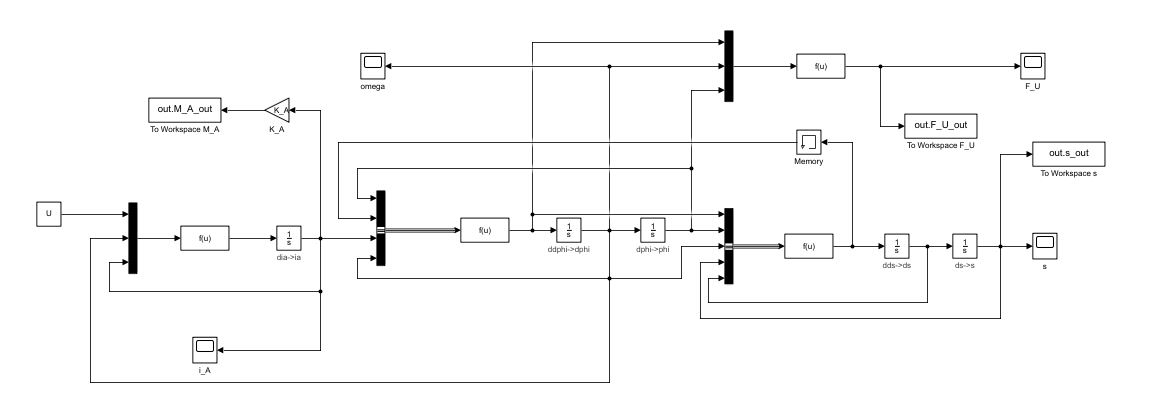
\includegraphics[width=1\linewidth]{Images/ProjektB_Elektrik_Blockdiagramm}
	\caption{SIMULINK Blockdiagramm zur Simulation des Systemverhaltens mit Memory-Block zur Umgehung der algebraischen Schleife}
	\label{fig:Blockdiagramm}
\end{figure}

Mithilfe von Scopes werden nun die gesuchten Signale abgegriffen und als Funktionen der Zeit dargestellt. \\
In der folgenden Abbildung sind Winkelgeschwindigkeit $\omega$, die Strecke $s$, der Strom $i_A$ und die Unwuchtkraft über die Zeit von $100 \milli\second$ dargestellt.

\begin{figure}[hbt]
	\centering
	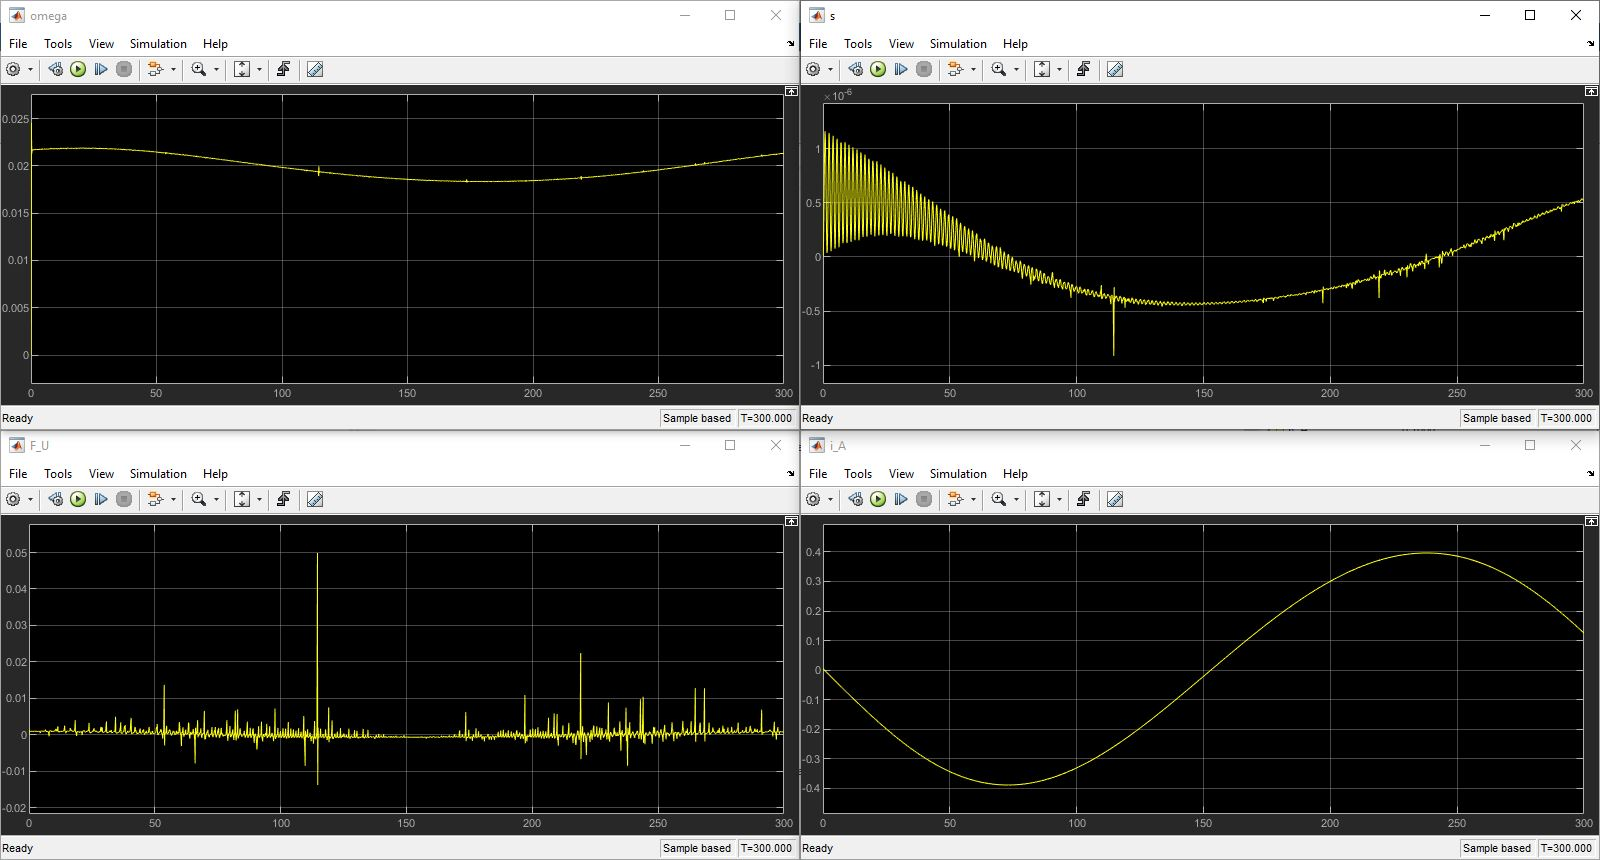
\includegraphics[width=0.5\linewidth]{Images/ProjektB_Elektrik_Diagramme_1}
	\caption{Winkelgeschwindigkeit $\omega$, Strecke $s$, Strom $i_A$ und Unwuchtkraft über die Zeit von $100 \milli\second$}
	\label{fig:Simulationsergebnisse}
\end{figure}


\chapter{Aufgabenteil b.)}
\begin{description}
	\item[b.)]
	Untersuchen Sie die Wechselwirkungen zwischen Schwingsystem und Gleichstrommotor. Bestimmen Sie hierfür die zeitlichen Verläufe des Antriebsmoments $M_A$, der Winkelgeschwindigkeit $\Omega$, der Unwuchtkraft $F_U$ und der Auslenkung $s$ des Systems.
\end{description}
\section{Simulationsergebnisse}


Mithilfe von Scopes oder Plots werden nun die gesuchten Signale abgegriffen und als Funktionen der Zeit dargestellt. \\
Die Abbildungen \ref{fig:Moment}, \ref{fig:Omega} und \ref{fig:StreckeundUnwuchtkraft} sind Plots aus Matlab, die wie folgt definiert wurden:

\begin{figure}[hbt]
	\centering
	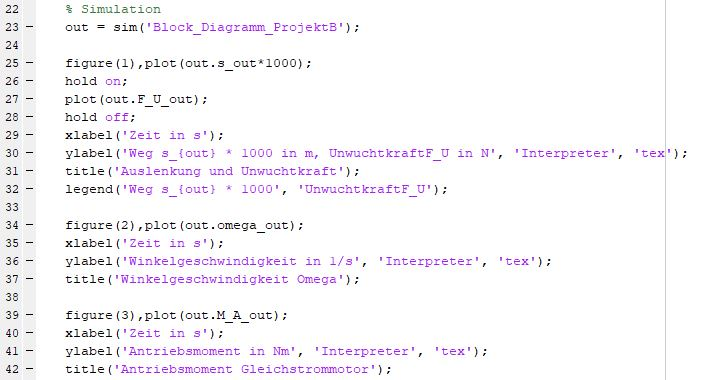
\includegraphics[width=1\linewidth]{Images/Simulationscode}
	\caption{Codeausschnitt aus dem Workspace zur Definition der Plots}
	\label{fig:Simcode}
\end{figure}

In den folgenden Abbildungen \ref{fig:Moment}, \ref{fig:Omega} und \ref{fig:StreckeundUnwuchtkraft} sind das Motormoment $M$, die Winkelgeschwindigkeit $\Omega$, die Strecke $s$ und die Unwuchtkraft $F_U$ über die Zeit von $100 \milli\second$ dargestellt. Für kleine Änderungen der Dämpfungskonstanten können die translatorischen und rotatorischen Bewegungsgleichungen getrennt betrachtet werden.

\begin{figure}[hbt]
	\centering
	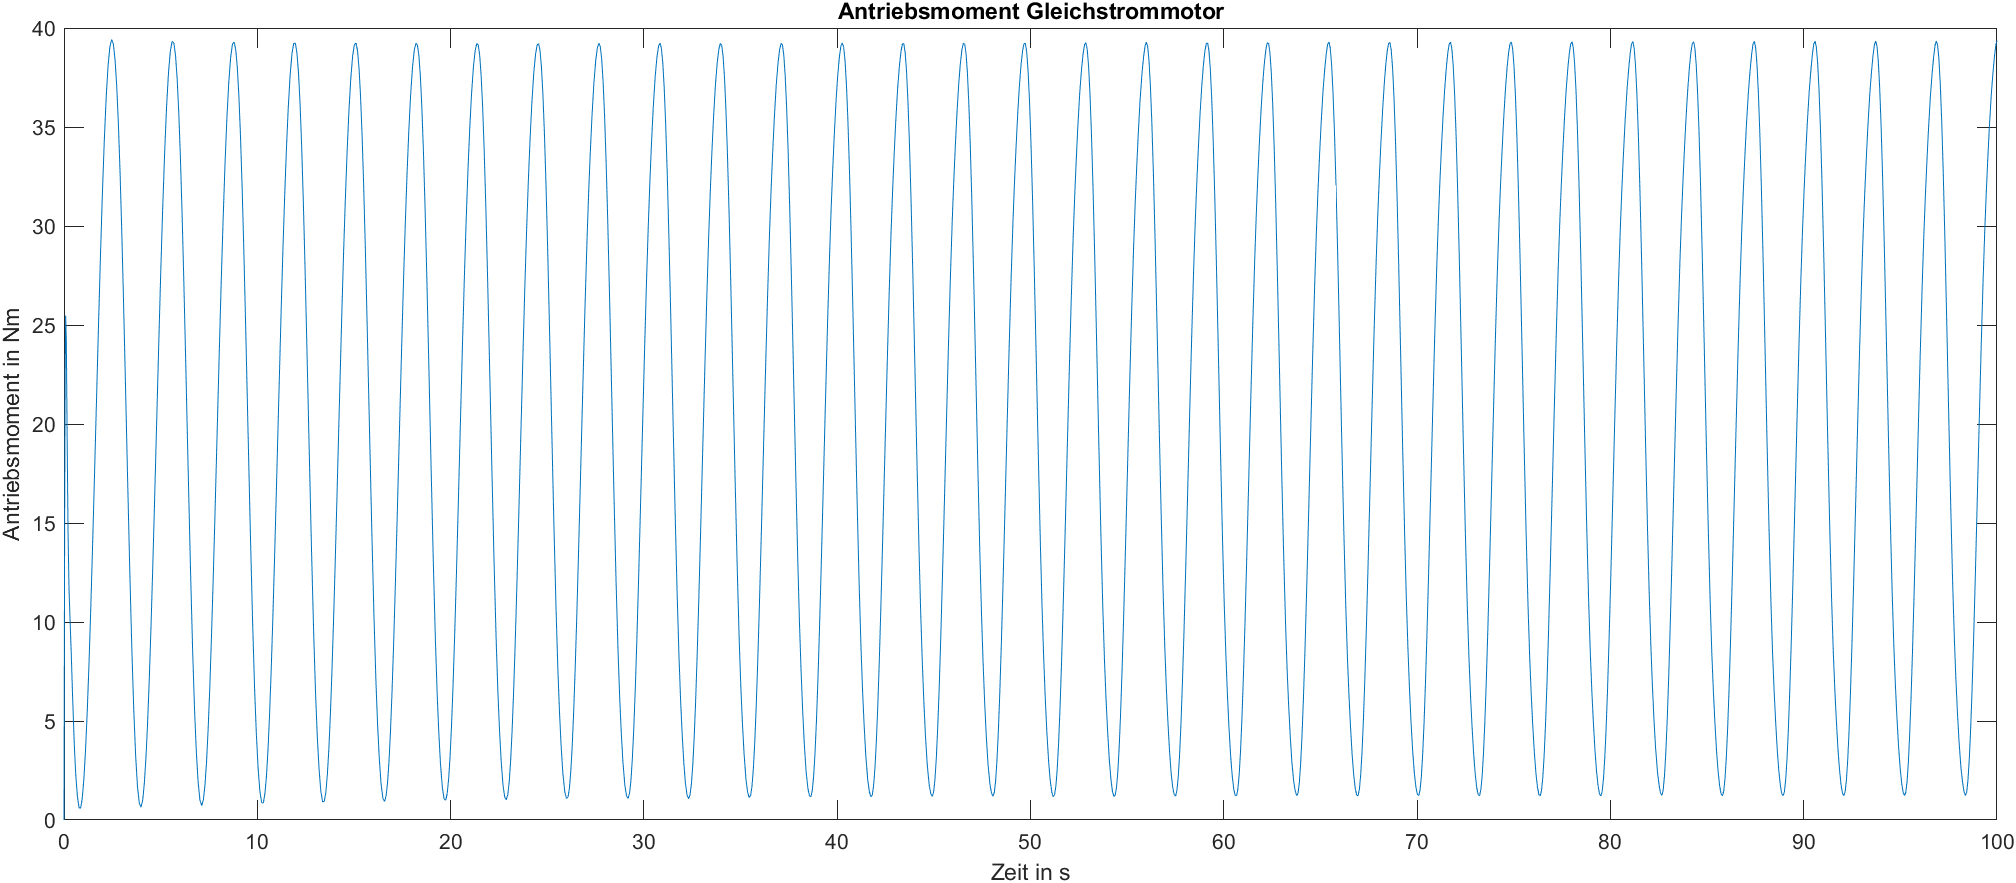
\includegraphics[width=1\linewidth]{Images/Moment}
	\caption{Simulationsergebnis: Antriebsmoment des Gleichstrommotors}
	\label{fig:Moment}
\end{figure}

Das in \ref{fig:Moment} dargestellte Antriebsmoment ist hauptsächlich abhängig von der rotatorischen Bewegungsgleichung des Schwingsystems, ebenso wie die Winkelgeschwindigkeit $\Omega$. Im Verlauf dieser beiden Größen und aus dem gegebenen Parametersatz kann dieses Teilsystem dem Schwingungsfall zugewiesen werden, dessen zeitlicher Verlauf auf eine ungedämpfte Schwingung deuten lässt und damit auch auf die Grenzstabilität des Systems. Zur genaueren Analyse, wird der Wert der rotatorischen Dämpfungskonstante $d_r$ verändert, um die Abhängigkeit von dieser zu überprüfen. 
Verdoppelt man den Wert von $d_r$ verschiebt sich die Amplitude des Antriebsmoments um $20 \newton\meter$ nach oben. Bei einer weiteren Erhöhung wird die Kurve ebenfalls immer weiter nach oben gerückt, wobei sich jedoch die Amplitude von $40 \newton\meter$ kaum verändert. \\ \\
Unter den Standardbedingungen befindet sich die Winkelgeschwindigkeit zwischen $1,85 \frac{1}{\second}$ und $2,18 \frac{1}{\second}$. Die Veränderungen an der Dämpfungskonstante $d_r$ hatten keinen nennenswerten Einfluss auf die Winkelgeschwindigkeit. Um diese marginal zu Beeinflussen müsste entweder die Motorkonstante $K_A$ angepasst werden, was sich wiederum auf das Antriebsmoment und die Unwuchtkraft auswirkt, oder $d_t$ wird größer gewählt wodurch der Maximalwert von $\Omega$ verkleinert wird. \\

\begin{figure}[hbt]
	\centering
	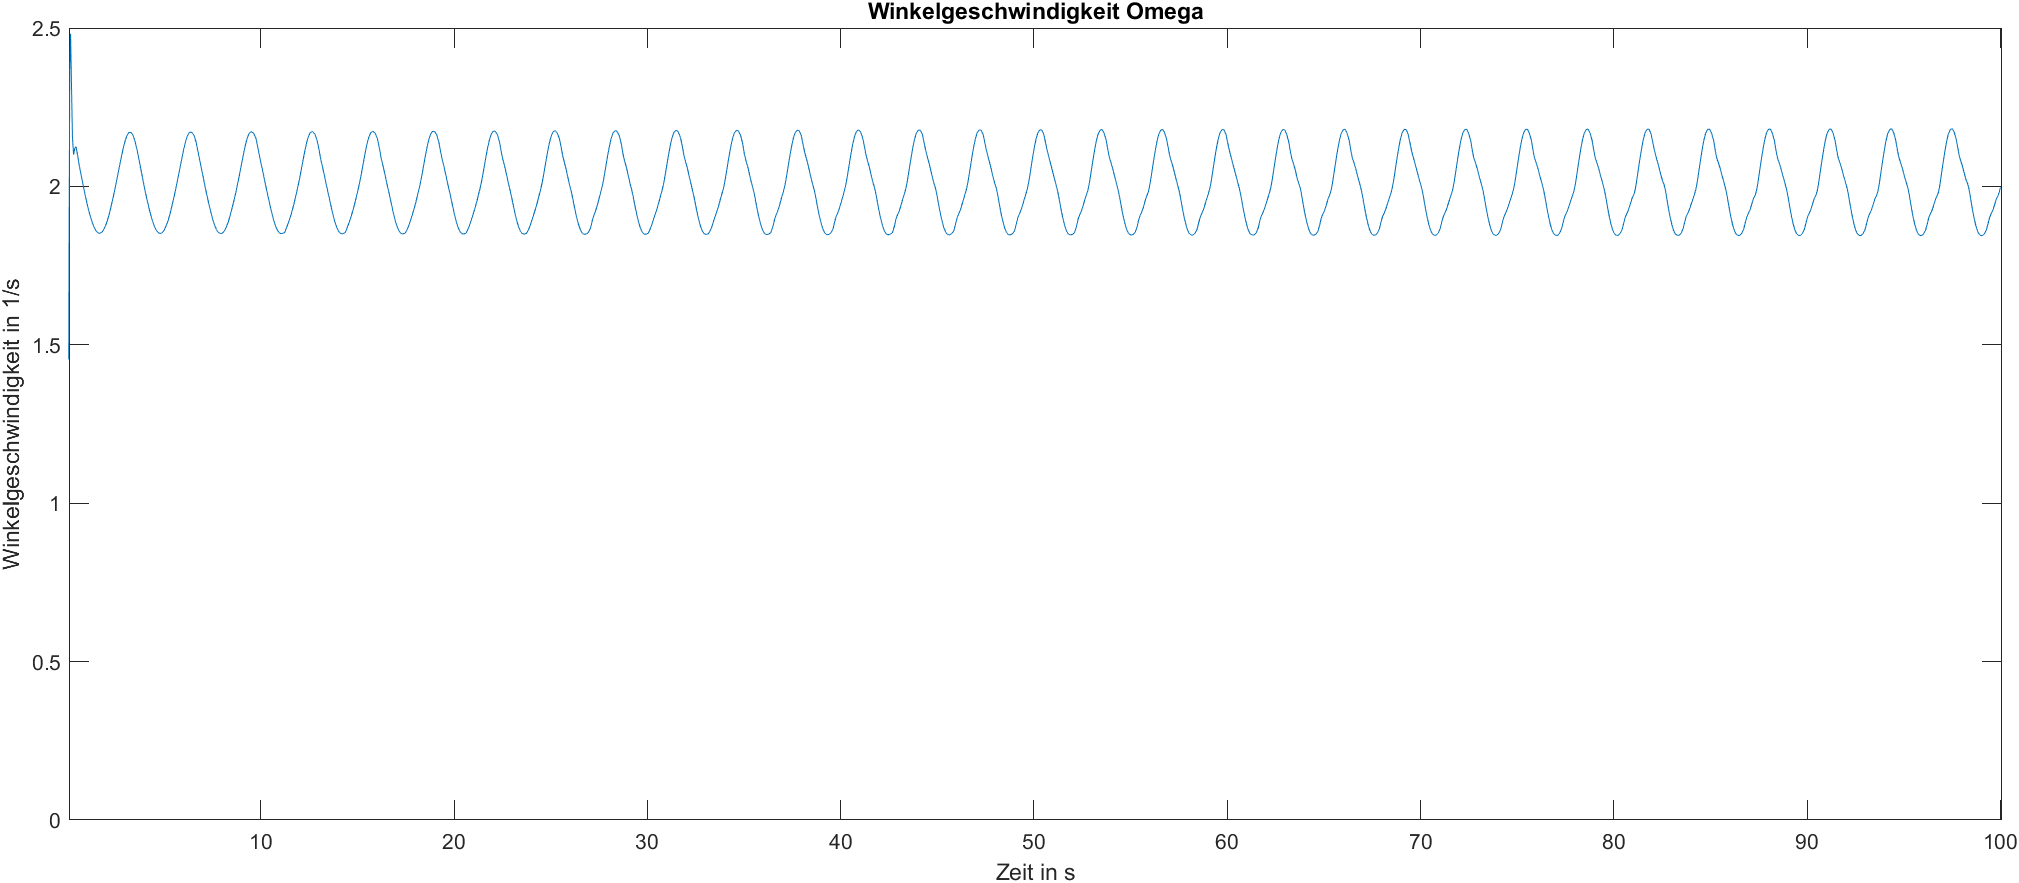
\includegraphics[width=1\linewidth]{Images/Omega}
	\caption{Simulationsergebnis: Winkelgeschwindigkeit des mechatronischen Systems}
	\label{fig:Omega}
\end{figure}

Auffällig ist in Abbildung \ref{fig:StreckeundUnwuchtkraft}, dass die Auslenkung die doppelte Frequenz der Unwuchtkraft hat.
Für die Auslenkung und Unwuchtkraft des Systems ist vor allem die translatorische Bewegungsgleichung verantwortlich. Aus Abbildung \ref{fig:StreckeundUnwuchtkraft} ist ersichtlich, dass es sich bei diesem Teilsystem um einen Schwingfall handelt. Im weiteren lässt der zeitliche Verlauf beider Kurven auf zwei unterschiedliche Schwingungsverhalten schließen. Die Amplitude der Auslenkung zeigt ein ungedämpftes Verhalten, wodurch diese Teilgleichung als instabil klassifiziert werden kann. Dahingegen zeigt der Graph von $F_U$ eine ungedämpfte Schwingung, bei gleichbleibender Amplitude und damit Eigenschaften eines grenzstabilen Systems. Um eine detailliertere Aussage über das translatorische System zu treffen wird dessen Dämpfungskonstante $d_t$ variiert.
\begin{figure}[hbt]
	\centering
	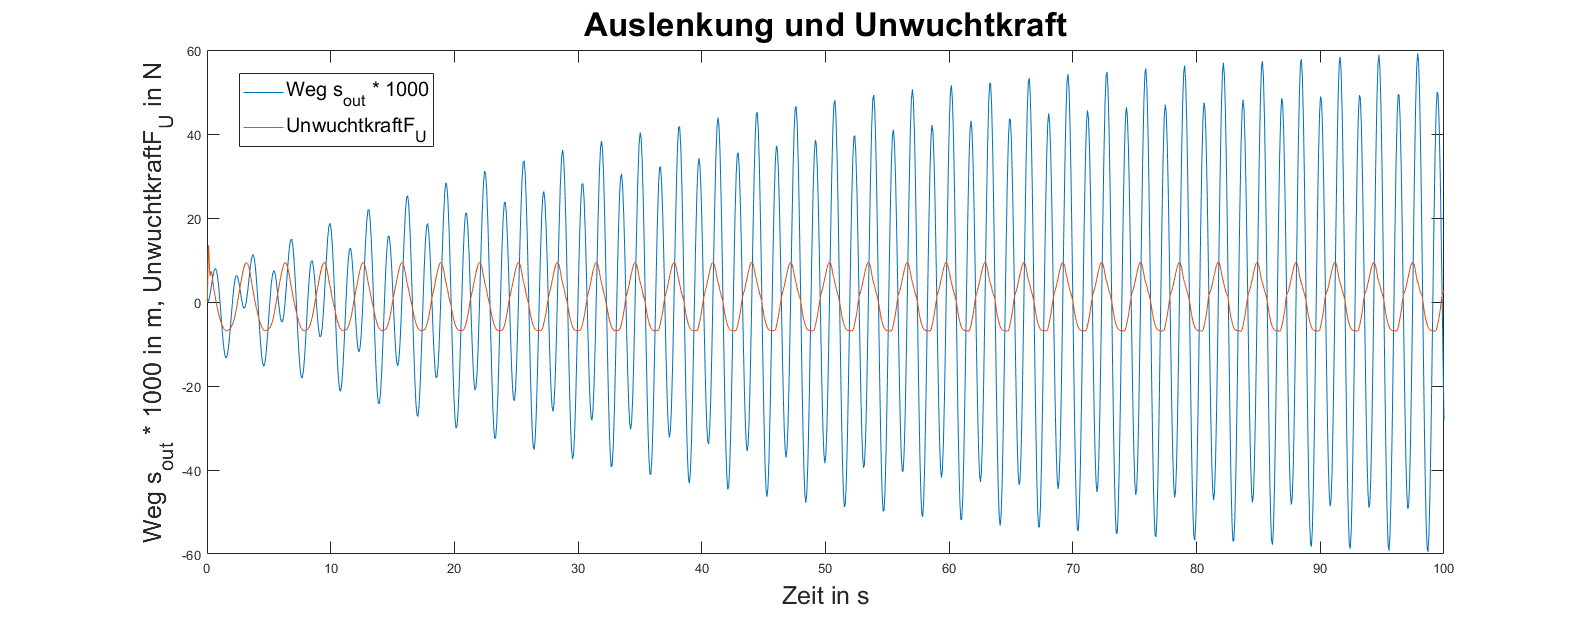
\includegraphics[width=1\linewidth]{Images/StreckeundUnwuchtkraft}
	\caption{Simulationsergebnis: Auslenkung$\cdot$1000 und Unwuchtkraft des mechatronischen Systems}
	\label{fig:StreckeundUnwuchtkraft}
\end{figure}
Für die Auslenkung und Unwuchtkraft des Systems ist vor allem die translatorische Bewegungsgleichung verantwortlich. Aus \ref{fig:StreckeundUnwuchtkraft} ist ersichtlich, dass es sich bei diesem Teilsystem um einen Schwingfall handelt. Im weiteren lässt der zeitliche Verlauf beider Kurven auf zwei unterschiedliche Schwingungsverhalten schließen. Die Amplitude der Auslenkung zeigt ein ungedämpftes Verhalten, wodurch diese Teilgleichung als instabil klassifiziert werden kann. Dahingegen zeigt der Graph von $F_U$ eine ungedämpfte Schwingung, bei gleichbleibender Amplitude und damit Eigenschaften eines grenzstabilen Systems. Um eine detailliertere Aussage über das translatorische System zu treffen, wird dessen Dämpfungskonstante $d_t$ variiert. Bei einer Erhöhung wird die Amplitude im gleichen Zeitbereich verkleinert. Je höher $d_t$ gewählt wird, desto kleiner wird die Amplitude der Auslenkung. Der resultierende Graph lässt darauf deuten, dass sich die Schwingung einem stabilen, ungedämpftem System annähert. Die Unwuchtkraft zeigt keine Reaktion auf die veränderten Werte der Dämpfungskonstante, ebenso wie $M_A$ und $\Omega$. \\ \\
Für beide Teilsysteme gilt, dass sie in erster Linie von ihren Dämpfungskonstanten abhängig sind und sich dadurch nicht marginal gegenseitig beeinflussen, solange diese nicht extrem groß werden. Lässt man $d_r$ gegen einen großen Wert laufen verkleinert sich die Amplitude von $F_U$, zugleich nähert sich der Auslenkungsgraph, dem von $F_U$ in Frequenz und Schwingungsverlauf an. Im anderen Teilsystem lässt sich beim Antriebsmoment keine Schwingung mehr erkennen, dieses läuft gegen einen Grenzwert. Vergleichbar vom Signalverlauf verhält sich auch die Winkelgeschwindigkeit, welche anfangs linear ansteigt und letztlich mit kleiner Amplitude um einen Wert schwingt. Wird $d_t$ sehr groß, hat das keine Auswirkungen auf $M_A$, $\Omega$ und $F_U$, nur die Auslenkung wird dadurch beeinflusst. Diese verhält sich ähnlich zur vorherigen Grenzbetrachtung und schmiegt sich zunächst $F_U$ an. Im weiteren Verlauf verringert sich die Amplitude der Auslenkung jedoch weiter und die der Unwuchtkraft bleibt gleich.

\chapter{Ausblick}
%Autor:

\label{Ausblick}



\chapter {Fazit}
%Fazit - Autor:
\label{Fazit}

Abschließend kann man sagen, dass es beim Handling mit Matlab einige Probleme aufgrund von fehlenden Kenntnissen und Erfahrungen gab. So war uns anfangs nicht bewusst, dass die Eingangsvariablen bei Matlab SIMULINK händisch mit einer Referenz auf die im Workspace deklarierten Variablen zu versehen sind. Nachdem wir das festgestellt und behoben haben, wurden die Plots zwar verändert, jedoch entsprachen sie nicht unseren Erwartungen. \\
Eine Überlegung war, die Eingangsvariable händisch innerhalb von Matlab SIMULINK zu verändern, sodass wir dann das richtige Ergebnis bezüglich der Graphen herausbekommen. Jedoch hätte dies nach unserer Bewertung das Ziel, den Sinn und damit das ganze Projektergebnis verfälscht, sodass wir uns darauf festgelegt haben diese Möglichkeit nicht in Betracht zu ziehen. \\
Das fehlen von Matlab-Packages war unser erster Verdacht. Nach einer kurzen Recherche, welche Packages benötigt werden und einem Vergleich mit den von uns heruntergeladenen Daten, konnten wir diese Möglichkeit ausschließen. \\
Auffällig war jedoch, als unser Programm auf einem anderen Laptop mit einer älteren Matlab Version das richtige Ergebnis hervorbrachte. Somit lag der nächste Verdacht nun auf der heruntergeladenen Matlab Version. \\
Während der Installation der älteren Matlab Version, setzten wir uns weiter mit unserem Programm und dem Aufbau des Quellcodes im Workspace auseinander. Auch die Schaltung in SIMULINK wurde weiter analysiert. Wir konnten so feststellen, dass aufgrund der Historie in Bezug auf die Referenzen der Variablen, einiges von Matlab verfälscht wurde. So veränderte SIMULINK die Eingangsvariable $U$, jedoch wurde diese einmalig abgespeichert, sodass Veränderungen nicht übernommen wurden. Die Ursache hierfür liegt darin, dass die von SIMULINK erstellte Variable, jene aus dem Workspace überschreibt. \\
Daher mussten wir uns die vom Model Explorer erstellten Variablen und deren Referenzen genauer anschauen. Wir löschten, die von Simulink erstellte Variable $U$ aus dem Speicher. Diese soll die Eingangsvariable aus dem Workspace nun nicht mehr überschreiben können, sodass der richtige Wert übernommen wird. \\
So haben wir es dann geschafft nach einiger Zeit, durch Analysieren, Recherchieren und Ausprobieren, Matlab SIMULINK mit dem Workspace zu verknüpfen und somit das Projekt erfolgreich durchzuführen. Das Installieren einer anderen Matlab Version war auch nicht mehr notwendig. \\

\addchap{Autorenverzeichnis}
\renewcommand\thesection{\arabic{section}}
Alexander Herrmann\\
Johannes Ruffer\\

\addchap{Verzeichnis verwendeter Abkürzungen und Formelzeichen}

\begin{acronym}%[CSMA/CD + AMP]
	
	\acro{DHBW}{Duale Hochschule Baden-Würtemberg}
	
\end{acronym}

% ---- Literaturverzeichnis ----------

\bibliography{Literatur/literatur}
										% Einbindung mehrerer Verzeichnisse in einem \bibliography Befehl mit Kommata trennen - keine Leerzeichen nach den Kommata!
\bibliographystyle{alphadin}           	%plain: alphabetisch, unsrt: nach Zitat, alphadin: NameJahr


% -----Ausgabe aller Verzeichnisse ---
\setlength{\parskip}{0.5\baselineskip}
\renewcommand{\indexname}{Sachwortverzeichnis}
\printindex								% Erzeugen des Indexverzeichnises
\addcontentsline{toc}{chapter}{\indexname}
% Version 0.1 vom 31.10.14 - T. Kibler

% Änderungswünsche bitte an T. Kibler melden

% alle Abkürzungen, die in der Arbeit verwendet werden. Nachfolgend sind allgemeine Abkürzungen aufgelistet. Die für die Arbeit spezifischen Abkürzungen sollten innerhalb des Haupttextes aufgeführt werden. Die Alphabetische Sortierung übernimmt Latex.

				% Datei mit allgemeinen Abkürzungen laden
%\renewcommand{\nomname}{Verzeichnis verwendeter %Formelzeichen und Abkürzungen}
%\setlength{\nomlabelwidth}{.20\hsize}
%\renewcommand{\nomlabel}[1]{#1 \dotfill}
%\setlength{\nomitemsep}{-\parsep}
%\printnomenclature						% Erzeugen des Abkürzungsverzeichnises, siehe auch Inhalt der Datei pages/abkuerzungen.tex
%\cleardoublepage
%\renewcommand{\glossaryname}{Glossar}
%\printglossaries
%\cleardoublepage
\listoffigures 							% Erzeugen des Abbildungsverzeichnisses 
\cleardoublepage
\listoftables 							% Erzeugen des Tabellenverzeichnisses
\cleardoublepage

% -----Anhang ------------------------
\appendix
\chapter{Anhang}

\section{Weitere Abbildungen}
%\clearpage
%\pagenumbering{Roman}					% große, römische Seitenzahlen für Anhang, falls gewünscht

\end{document}